\section{Evaluation} \label{evaluation}
When evaluating the success of a project, it is paramount to keep in mind the original goals of the project.
In this case, the primary goal was to provide an alternative VM emulator implementation to the participants of the Nand to Tetris course to make Project 9 and 12 more convenient.
Not only was this goal achieved, but in addition, the CPU emulator was also rewritten and both emulators have been integrated into a test-script-driven workflow, making them useful to course instructors.
Then again, projects do not exist in a vaccum, so the following sections contain a comprehensive comparison with the official emulator.

\subsection{Comparison with the official Emulator based on compatability} \label{compatibility}
It is impossible to test every existing program for the Hack VM, both due to the sheer volume of existing applications and the fact that many of these applications are not available to the public.
However, this is also not necessary, since the expected behavior of the emulators is clearly described in the book accompanying the course.
By following the specification and testing the new implementation with a reasonable number of representative programs, one can determine the degree of compatibility.
Those programs are listed in the appendix~\ref{table:tested}.
The number of possible instructions in the VM is also manageable, so a sufficiently complex program will use every single available instruction, which further supports this claim.
Additionally, the course materials include a variety of test cases to help users implement the Jack compiler.
These tests were used to further verify the correct behavior of the new VM implementation.
By and large, the new emulator behaves exactly like the old one.
This even applies to behaviors that could be considered bugs, such as the way the keyboard handler in the Java implementation interprets each letter as a capital letter, thus limiting the entire input system to uppercase letters.
This is not a technical limitation of either the VM or the Java input event, but simply a consequence of the implementation of the keyboard handler, and could easily be changed to allow lowercase letters as well.
But that would affect a number of existing applications, since they only check for uppercase letters in their game code, which means that those applications could no longer be used without problems.
For this reason, the new emulator also only passes uppercase letters to the VM, even if it needs a bit more code to behave that way.
All keys are converted directly to uppercase after being read.
In the future, it might be useful to add a compatibility setting to allow users to process lowercase letters as well, but due to the time constraints of this project, it was decided to prioritize compatibility over correctness.
There is only a single part of the new emulator that is known to behave at least partially differently to the official implementation.
That is the implementation of the \verb+Sys.wait+ function, which was already discussed in~\cref{sys.wait-example}.

% \begin{itemize}
%   \item every program working. systematic approach because there are tons of non public programs. Example programs that use every instruction/stdlib-function
%   \item Sys.wait not the same (but also different behaviour on official emulator, based on stdlib)
%   \item Sys.wait behaves differently in vm stdlib on official emulator
%   \item keyboard bug for bug compatible
% \end{itemize}

\subsection{Comparison with the official Emulator based on UI} \label{ui-compatibility}
The new emulator does not implement all the features of the official emulator.
Some of these missing features are missing due to time constraints, such as test script support in the WebUI~\ref{future-work}.
On the other hand, some features have been deliberately omitted because they serve little purpose but complicate the user interface.
One such feature is the ability to animate the running program.
When this option is enabled, the information about the internal memory and the current instruction is updated after each tick.
Everytime one of those values changes, it is highlighted in the UI.
This may seem useful at first, but while debugging, the user will usually use the step button instead, and when running the game, the animations have to be disabled for performance reasons.
Thus, this feature does not offer much benefit to the user.
Instead of offering every possible feature, the new user interface is intentionally kept minmal to simplify usage and provide an experience that is more focused on actually running games at full speed.
This is also the reason why most of the UI elements are completely hidden while the game is running.
For the compiler development that is part of projects 10 and 11, it may be advantageous to continue using the official emulators for their advanced debugging features.
In contrast, when it comes to playing and testing full games, the new emulators offer a superior experience.
They also open up these games and programs to additional platforms, because the new emulators also work on phones and tablets, as long as a physical keyboard is connected or the application does not require user input~\ref{fig:ui-demo-mobile}.
Another benefit of the new user interface is the unification of the VM and CPU emulators.
The new emulator handles both types of applications within a single application, distinguishing between them based on their respective file extensions.
% \begin{itemize}
%   \item official has more features (including test scripts)
%   \item mine scales better
%   \item mine is available in the browser -> also on mobile
%   \item mine handles cpu and vm in one ui
% \end{itemize}

% \subsubsection{Hosting the application}

\subsection{Comparison with the official Emulator based on Performance} \label{sec:benchmarks}
There are two distinct modes in which the emulators can operate: interactive mode, in which the display memory is actually rendered onto a visible canvas, and test mode, in which a test script runs without further user input to verify the correctness of a VM or CPU program.
From a performance point of view, only the former is relevant, since all test scripts used in the course finish so quickly that measuring the performance differences between emulators would basically be meaningless.
So, to really evaluate the new emulators, a sufficiently complex graphical program is required.
For this task, one of Gavin Stewart's impressive graphical demonstrations for the Hack platform was chosen.
The GASchunky program~\cite{demos} renders a complex animation in an infinite loop to the internal display.
It requires no user input, but uses almost all of the available functionality of the platform, making it a perfect choice for benchmarking.
Since the number of instructions and standard library functions is relatively small, a single complex program can adequately represent the speed of the entire platform.
In order to turn it into a proper benchmark, the loop was removed, leaving only a single iteration of the animation to be played.
\cref{fig:gaschunky-screenshot} shows a frame of the generated animation.
Additionally, to make the comparisons fair, all \verb+Sys.wait+ calls have been removed from the program.
The reason why this is important was discussed at the end of \cref{sys.wait-example}.
\begin{center}
  \begin{figure}[ht]
    \centering
    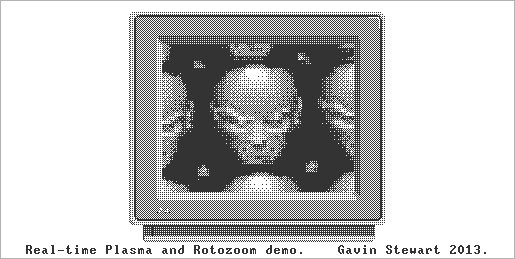
\includegraphics[width=10cm]{fig/gaschunky.png}
    \caption{A screenshot of the GASchunky animation in progress.}%
    \label{fig:gaschunky-screenshot}
  \end{figure}
\end{center}
There were also some changes made to the emulators themselves.
Two statements have been added to the code for both the official and the new emulator.
Both print the current system time in milliseconds and get executed when the start button is pressed and when the program returns from the main function respectively.
Additionally in the ``Official (no wait)'' column of the ~\cref{table:gaschunky}, the one millisecond wait instruction in the FastforwardTask of the \verb+HackController.java+ was removed to ensure that the official emulator could run at its maximum speed.
The new emulator was run both from the web UI and in desktop mode.
For the ``Native'' and ``Linux 10x Firefox'' columns, the tick rate has been set to one million, instead of the default maximum tick rate of one hundred thousand in the web UI.
This normal maximum of 100,000 is arbitrarily chosen and therefore does not reflect the true performance of the system.
At a tick rate of one million, the viewer can still see the animation clearly, which allows for a fair comparison~\ref{fig:gachunky-plot}.
That said, the other four columns for both Linux and Windows use this arbitrary limit because that is the experience users will have by default.
This limit was chosen to ensure that games developed for the official emulator run at a reasonable speed by default and are neither too fast nor too slow.

\begin{table}[ht]
  \begin{tabular}{c p{1.5cm} c p{1.7cm} p{1.5cm} p{1.5cm} p{1.5cm} p{1.5cm}}
    \toprule
    Official & Official (no wait) & Native & Linux 10x Firefox & Linux Firefox & Linux Chrome  & Windows Firefox & Windows Chrome\\
    \midrule
    36.16s &             30.76s &  1.01s & 1.02s               & 2.91s         & 5.68s         & 10.39s           & 3.43s          \\
    36.19s &             31.17s &  0.99s & 1.03s               & 2.92s         & 5.66s         & 10.39s           & 3.47s          \\
    35.93s &             30.58s &  1.02s & 1.04s               & 2.81s         & 5.59s         & 10.39s           & 3.51s          \\
    36.14s &             30.65s &  0.97s & 1.06s               & 2.81s         & 5.80s         & 10.39s           & 3.54s          \\
    36.16s &             30.99s &  0.95s & 1.02s               & 2.81s         & 5.38s         & 10.40s           & 3.49s          \\
    36.12s &             30.81s &  1.03s & 1.07s               & 2.87s         & 5.39s         & 10.38s           & 3.51s          \\
    36.27s &             30.86s &  1.06s & 1.06s               & 2.95s         & 5.38s         & 10.36s           & 3.54s          \\
    36.29s &             30.86s &  0.99s & 1.05s               & 2.95s         & 5.39s         & 10.38s           & 3.49s          \\
    35.86s &             30.81s &  1.01s & 1.03s               & 2.94s         & 5.36s         & 10.39s           & 3.39s          \\
    36.12s &             30.74s &  1.02s & 1.04s               & 2.91s         & 5.45s         & 10.29s           & 3.43s          \\
    \bottomrule
  \end{tabular}
  \caption{GASchunky benchmark in seconds (lower is faster).}%
  \label{table:gaschunky}
\end{table}

\begin{figure}[ht]
  \centering
  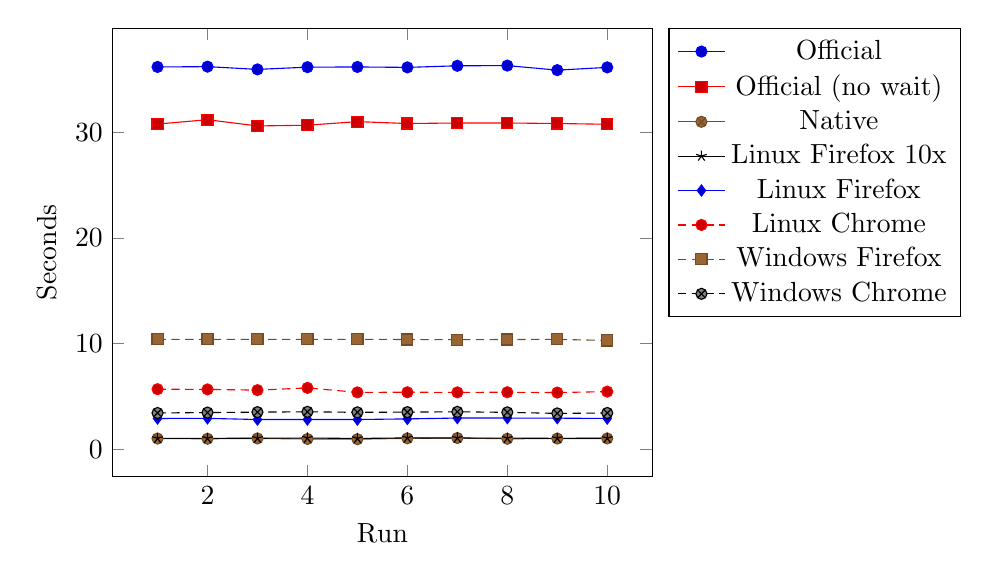
\begin{tikzpicture}
    \begin{axis}[
      % ymode=log,
      ylabel=Seconds,
      xlabel=Run,
      legend pos=outer north east,
      ]
      \addplot coordinates {
        (1,  36.16)
        (2,  36.19)
        (3,  35.93)
        (4,  36.14)
        (5,  36.16)
        (6,  36.12)
        (7,  36.27)
        (8,  36.29)
        (9,  35.86)
        (10, 36.12)
      };
      \addplot coordinates {
        (1,  30.76)
        (2,  31.17)
        (3,  30.58)
        (4,  30.65)
        (5,  30.99)
        (6,  30.81)
        (7,  30.86)
        (8,  30.86)
        (9,  30.81)
        (10, 30.74)
      };
      \addplot coordinates {
        (1,  1.01)
        (2,  0.99)
        (3,  1.02)
        (4,  0.97)
        (5,  0.95)
        (6,  1.03)
        (7,  1.06)
        (8,  0.99)
        (9,  1.01)
        (10, 1.02)
      };
      \addplot coordinates {
        (1,  1.02)
        (2,  1.03)
        (3,  1.04)
        (4,  1.06)
        (5,  1.02)
        (6,  1.07)
        (7,  1.06)
        (8,  1.05)
        (9,  1.03)
        (10, 1.04)
      };
      \addplot coordinates {
        (1,  2.91)
        (2,  2.92)
        (3,  2.81)
        (4,  2.81)
        (5,  2.81)
        (6,  2.87)
        (7,  2.95)
        (8,  2.95)
        (9,  2.94)
        (10, 2.91)
      };
      \addplot coordinates {
        (1,  5.68)
        (2,  5.66)
        (3,  5.59)
        (4,  5.80)
        (5,  5.38)
        (6,  5.39)
        (7,  5.38)
        (8,  5.39)
        (9,  5.36)
        (10, 5.45)
      };
      \addplot coordinates {
        (1,  10.39)
        (2,  10.39)
        (3,  10.39)
        (4,  10.39)
        (5,  10.40)
        (6,  10.38)
        (7,  10.36)
        (8,  10.38)
        (9,  10.39)
        (10, 10.29)
      };
      \addplot coordinates {
        (1,  3.43)
        (2,  3.47)
        (3,  3.51)
        (4,  3.54)
        (5,  3.49)
        (6,  3.51)
        (7,  3.54)
        (8,  3.49)
        (9,  3.39)
        (10, 3.43)
      };
      \addlegendentry{Official}
      \addlegendentry{Official (no wait)}
      \addlegendentry{Native}
      \addlegendentry{Linux Firefox 10x}
      \addlegendentry{Linux Firefox}
      \addlegendentry{Linux Chrome}
      \addlegendentry{Windows Firefox}
      \addlegendentry{Windows Chrome}
    \end{axis}
  \end{tikzpicture}
  \caption{GASchunky benchmark (lower is faster).}%
  \label{fig:gachunky-plot}
\end{figure}

It can be clearly seen that the performance of the new emulator, while very much dependent on the particular web browser and operating system, is consistently several times faster than the official implementation.
On average, the official emulator without modifications takes around 36 seconds to render the full animation once.
The web version of the new emulator can achieve the same result in just one second on average when the artificial upper limit for the tick rate is removed.
The native version of the new emulator, which uses SDL to render the internal display, is even slightly faster.
While the official emulator can be sped up drastically, it still does not come close.
This shows us that even though the new emulator only uses a single thread and runs in a browser, it still offers massive performance benefits over the official implementation.
It is worth noting that not only the browser is relevant for the final performance, but also the combination of browser and operating system.
